\documentclass[a4paper,10pt]{article}
\usepackage[utf8]{inputenc}
\usepackage[spanish]{babel}
\usepackage[affil-it]{authblk}
\usepackage{enumerate}
\usepackage{graphicx}
\usepackage{hyperref}
\usepackage{amsmath}
\usepackage{amssymb}
\usepackage{cancel}
\usepackage[usenames, dvipsnames]{color}
\usepackage{tikz}
\usepackage[labelfont=bf]{caption}
\usepackage{subcaption} %Multiple images
\usepackage{multicol} % Multiple columns
\usepackage{float}
\usepackage{cleveref}
 \usepackage{relsize} % bigger math symbols
\usepackage[margin=1.4in]{geometry}
\usepackage[titletoc,toc,title]{appendix}
\usepackage{enumitem}
\usepackage{etoolbox}
\usepackage{mdframed} %frame theorems
\usetikzlibrary{calc}
\numberwithin{equation}{section}

% Enviroment for theorems
\newmdtheoremenv[frametitle=Teorema]{theo}{Theorem}

% Circled words
\newcommand{\circled}[2][]{%
  \tikz[baseline=(char.base)]{%
    \node[shape = circle, draw, inner sep = 1pt]
    (char) {\phantom{\ifblank{#1}{#2}{#1}}};%
    \node at (char.center) {\makebox[0pt][c]{#2}};}}
\robustify{\circled}

%Appendices in spanish
\renewcommand{\appendixname}{Ap\'endices}
\renewcommand{\appendixtocname}{Ap\'endices}
\renewcommand{\appendixpagename}{Ap\'endices}

%Zero delimiter
\newcommand{\zerodel}{.\kern-\nulldelimiterspace}

%Columns separation
\setlength{\columnsep}{1cm}

%Indentation
\setlength{\parindent}{0ex}

%Multiple References

\crefrangelabelformat{equation}{(#3#1#4--#5\crefstripprefix{#1}{#2}#6)}

\usepackage{xparse}

%Boxes

\newcommand*{\boxcolor}{blue}
\makeatletter
\renewcommand{\boxed}[1]{\textcolor{\boxcolor}{%
\tikz[baseline={([yshift=-1ex]current bounding box.center)}] \node [rectangle, minimum width=1ex,rounded corners,draw] {\normalcolor\m@th$\displaystyle#1$};}}
 \makeatother

%Constantes
\newcommand{\euler}{\mathrm{e}}
\newcommand{\im}{i}

%Lemas, teoremas, definiciones y pruebas
\newcommand{\definicion}{\textbf{Definición: }}
\newcommand{\lema}{\textbf{Lema: }}
\newcommand{\teorema}{\textbf{Teorema: }}
\newcommand{\prueba}{\textbf{Prueba: }}
\newcommand{\proposicion}{\textbf{Proposición: }}
\newcommand{\corolario}{\textbf{Corolario: }}

% Definición de las secciones y su numeración

\makeatletter
\def\@seccntformat#1{%
  \expandafter\ifx\csname c@#1\endcsname\c@section\else
  \csname the#1\endcsname\quad
  \fi}
\makeatother

%opening
\title{Electrodinámica Clásica. Tarea \# 2}
\author{Favio Vázquez\thanks{Correo: favio.vazquezp@gmail.com}}\affil{Instituto de Ciencias Nucleares. Universidad Nacional Autónoma de México.}
\date{}
\begin{document}

\makeatletter
\def\@maketitle{%
  \newpage
  \null
  \vskip 2em%
  \begin{center}%
  \let \footnote \thanks
    {\Large\bfseries \@title \par}%
    \vskip 1.5em%
    {\normalsize
      \lineskip .5em%
      \begin{tabular}[t]{c}%
        \@author
      \end{tabular}\par}%
    \vskip 1em%
    {\normalsize \@date}%
  \end{center}%
  \par
  \vskip 1.5em}
\makeatother

\maketitle

\section{Problema 1. Problema 2.1 de Classical Electrodynamics (tanto en la 2da 
como en la 3ra edición) de Jackson \cite{jackson2,jackson3}.}

Una carga puntual $q$ es llevada a una posición a una distancia $d$ desde un 
plano conductor infinito que está a un potencial cero. Usando el método de imágenes, 
encuentre: 

\begin{enumerate}[label=\textbf{(\alph*)}]
 \item la densidad de carga superficial inducida en el plano, y grafíquela;
 \item la fuerza entre el plano y la carga usando la ley de Coulomb para la fuerza 
 entre la carga y su imagen;
 \item la fuerza total actuando en el plano integrando $\sigma^2/2\epsilon_0$ 
 sobre todo el plano;
 \item el trabajo necesario para remover la carga $q$ de su posición al infinito;
 \item la energía potencial entre la carga $q$ y su imagen [compare la respuesta 
 con la de la parte (d) y discuta].
 \item Encuentre la respuesta a la parte (d) en eV para un electrón originalmente 
 a un angstrom de la superficie.
\end{enumerate}

\vspace{.3cm}

\underline{Solución:} \vspace{.3cm}

De la simetría del problema, debe ser claro que el potencial $\Phi$ debe ser equivalente 
al producido por una carga $q$, junto con una carga imagen $q' = -q$ a una distancia 
$d$ del lado opuesto del plano. Entonces el potencial debido a dos cargas puntuales 
una en $d$ de carga $q$ y una en $-d$ de carga $-q$ puede escribirse como:

\begin{equation}
 \Phi = \frac{q}{4\pi\epsilon_0}\left[\frac{1}{\sqrt{x^2+y^2+(z-d)^2}} 
 - \frac{1}{\sqrt{x^2+y^2+(z+d)^2}} \right].
\end{equation}

\textbf{(a)} La densidad de carga superficial puede encontrarse con la 
relación\footnote{Ecuación (2.5) de Jackson \cite{jackson3}.} 

\begin{equation}
 \left\zerodel \sigma = -\epsilon_0\frac{\partial\Phi}{\partial n}\right|_{S},
\end{equation}

\begin{equation}
 \left\zerodel \sigma = -\epsilon_0\frac{\partial\Phi}{\partial z}\right|_{z=0},
\end{equation}

\begin{equation}
  \left\zerodel \sigma = -\epsilon_0\frac{q}{4\pi\epsilon_0}\left[\frac{-(z-d)}{[x^2+y^2+(z-d)^2]^{3/2}} 
  + \frac{(z+d)}{[x^2+y^2+(z+d)^2]^{3/2}}\right]\right|_{z=0},
\end{equation}

Y evaluando en $z=0$ obtenemos 

\begin{equation}
 \boxed{\sigma = - \frac{1}{2\pi}\frac{qd}{(x^2+y^2+d^2)^{3/2}}}.
\end{equation}

\textbf{(b)} Calculemos usando la ley de Coulomb la fuerza entre la  carga y 
su imagen. Es fácil ver al usar la ecuación $Q = \int \sigma dA$ 
que la carga total inducida es $-q$ \cite{griffiths}, por lo tanto podemos decir que la carga $q$ 
es atraída hacia al plano, con carga inducida $-q$. Debido a que el potencial
en la vecindad de $q$ es la misma que en el problema análogo con el método de 
imágenes (el problema que nos planteamos de una carga $+q$ y una $-q$ sin el plano 
conductor), la fuerza será simplemente 

\begin{equation}
 \boxed{\mathbf{F} = - \frac{1}{16\pi\epsilon_0}\frac{q^2}{d^2}\hat{z}}.
\end{equation}

\textbf{(c)} La fuerza en el plano conductor debe ser igual y opuesta a la fuerza 
que calculamos en el inciso anterior. El texto nos solicita que hagamos este cálculo 
de forma independiente del anterior inciso, integrando $\sigma^2/2\epsilon_0$ sobre 
todo el plano. 

\vspace{.3cm}

La fuerza incremental por unidad de área se define como la presión electrostática, 

\begin{equation}
 \frac{d\mathbf{F}}{dA} = \sigma\mathbf{E},
\end{equation}

donde $\sigma$, que es la cantidad de proporcionalidad, es la densidad de carga 
inducida en el plano que calculamos en el inciso (a). Ahora, el campo eléctrico 
también está relacionado con $\sigma$ de acuerdo a 

\begin{equation}
 \mathbf{E} = \frac{\sigma}{2\epsilon_0}\hat{n},
\end{equation}

y usando estas ecuaciones encontramos la relación conocida para la presión electrostática 
en la superficie de un conductor, 

\begin{equation}
  \frac{d\mathbf{F}}{dA} = \frac{\sigma^2}{2\epsilon_0}\hat{n}.
\end{equation}

La fuerza total es simplemente la presión electrostática por un infinitesimal de 
área, 

\begin{equation}
 d\mathbf{F} = \frac{\sigma^2}{2\epsilon_0}\hat{n}dA,
\end{equation}

y sustituyendo la $\sigma$ que encontramos en (a), obtenemos 

\begin{align*}
 \mathbf{F} &= \frac{q^2d^2}{8\pi^2\epsilon_0}\int 
 \frac{rdrd\theta}{(x^2+y^2+d^2)^{3/2}} \hat{z}, \\
%
  &= \frac{q^2d^2}{8\pi^2\epsilon_0}\int 
 \frac{du\theta}{u^{3/2}}\hat{z}, \\
 %
 &= - \frac{q^2d^2}{16\pi\epsilon_0}\left\zerodel\frac{1}{u^2}\right|_{d^2}^\infty\hat{z}, \\
 %
 &= \frac{q^2d^2}{16\pi\epsilon_0d^4}\hat{z},
\end{align*}

\begin{equation}
 \boxed{\therefore \mathbf{F} = \frac{1}{16\pi\epsilon_0}\frac{q^2}{d^2}\hat{z}}.
\end{equation}

La cual es exactamente igual y opuesta a la fuerza que encontramos en el inciso 
anterior, como fue anticipado.

\vspace{.3cm}

\textbf{(d)} Para calcular el trabajo necesario para remover la carga $q$ de su 
posición al infinito, usamos la ecuación 

\begin{equation}
 W = \int_d^\infty \mathbf{F}(l)\cdot d\mathbf{l} = \frac{q^2}{16\pi\epsilon_0}
 \int_d^\infty \frac{dz}{z^2} = \left\zerodel 
 - \frac{q^2}{16\pi\epsilon_0} \frac{1}{z}\right|_d^\infty,
\end{equation}

\begin{equation}
 \boxed{\therefore W = \frac{q^2}{16\pi\epsilon_0d}}.
\end{equation}

\textbf{(e)} La energía potencial entre la carga y su imagen se calcula 
con la ecuación 

\begin{equation}
 U = \frac{q_1q_2}{4\pi\epsilon_0|r_1 - r_2|} = \frac{(q)(-q)}{4\pi\epsilon_0(2d)},
\end{equation}

\begin{equation}
 \boxed{\therefore U = - \frac{q^2}{8\pi\epsilon_0d}}.
\end{equation}

Vemos entonces que la energía cinética es exactamente el doble de energía requerida 
para remover la carga de su posición al infinito, que fue lo que calculamos en el 
inciso anterior. Esto es debido a que en el sistema original, solo existe el 
campo eléctrico debido a la partícula $q$, mientras en el problema que planteamos 
por el método de imágenes también está la energía de la partícula imagen; es decir, 
el problema real solo llena medio espacio $z>0$, mientras el problema con imágenes 
el campo llena todo el espacio y es simétrico sobre el origen $z=0$. Esto no dice que, 
genéricamente, los cálculos de energía electrostática no son directamente transferibles 
entre problemas reales a problemas resueltos con el método de imágenes.

\vspace{.3cm}

\textbf{(f)} Ahora calculemos, como es solicitado, la energía potencial utilizando 
la expresión del inciso (d) en eV para un electrón a un ansgtrom de la superficie.

\begin{equation}
 W = \frac{q^2}{16\pi\epsilon_0d} = \frac{(\text{e}^-)^2}{16\pi(5.526\times 10^7 \text{ e/Vm})
 (10^{-10}\text{ m})},
\end{equation}

\begin{equation}
 \boxed{W = 3.6 \text{ eV}}.
\end{equation}

\section{Problema 2. Problema 2.2 de Classical Electrodynamics (tanto en la 2da 
como en la 3ra edición) de Jackson \cite{jackson2,jackson3}.}

Usando el método de imágenes, discuta el problema de una carga puntual $q$ 
\emph{adentro} de una esfera hueca, conectada a tierra, conductora de radio interno
$a$. Encuentre 

\begin{enumerate}[label=\textbf{(\alph*)}]
 \item el potencial adentro de la esfera;
 \item la densidad de carga superficial inducida;
 \item la magnitud y dirección de la fuerza actuando sobre $q$.
 \item ¿Hay algún cambio en la solución si la esfera es mantenida a un potencial 
 fijo $V$? ¿y si la esfera tiene una carga total $Q$ en sus superficies internas y 
 externas?
\end{enumerate}

\vspace{.3cm}

\underline{Solución:} \vspace{.3cm}

Este problema es similar al discutido en la sección 2.2 de Jackson \cite{jackson3}, 
solo que en ese caso la carga estaba afuera de la esfera, pero los argumentos que 
utilizaremos para resolver este problema son muy similares a los que se presentan 
en esa sección. 

\vspace{.3cm}

\textbf{(a)} Si colocamos la carga en el punto $r$, entonces, por 
simetría axial, la carga imagen debe estar localizada a lo largo de la dirección 
de $r$ a una distancia $r' > a$. Por lo tanto, el potencial a un punto $\mathbf{x}$ será 

\begin{equation}
 \Phi(\mathbf{x}) = \frac{1}{4\pi\epsilon_0}\left(\frac{q}{|\mathbf{x}-\mathbf{r}|} + 
 \frac{q'}{|\mathbf{x}-\mathbf{r}'|} \right).
\end{equation}

Como lo explica el libro, debido a que la esfera está puesta a tierra, debe cumplirse 
que $\Phi(|\mathbf{x}| = a) = 0$. Y tenemos también como en el ejemplo del libro 
que 

\begin{equation}
 \frac{q}{a} = - \frac{q'}{r'} \qquad \text{y} \qquad \frac{r}{a} = \frac{a}{r'},
\end{equation}

entonces el potencial será (utilizando la ley del coseno)

\begin{equation}
 \boxed{\Phi(x) = \frac{q}{4\pi\epsilon_0}\left[\frac{1}{(x^2+r^2-2xr\cos{\gamma})^{1/2}}
 - \frac{a}{r(x^2+\frac{a^4}{r^2}-2x\frac{a^2}{r}\cos{\gamma})^{1/2}}\right]},
\end{equation}

donde $\gamma$ es el ángulo entre $\mathbf{r}$ y $\mathbf{x}$.

\vspace{.3cm}

\textbf{(b)} Para calcular la densidad de carga superficial inducida en la esfera, 
calculamos la derivada normal de $\Phi$ en en la superficie:

\begin{equation}
 \boxed{\sigma = -\epsilon_0\left\zerodel\frac{\partial \Phi}{\partial x}\right|_{x=a} = 
 \frac{q}{4\pi a r}\frac{1 - \frac{a^2}{r^2}}{\left(1 + \frac{a^2}{r^2} - 
 2\frac{a}{r}\cos{\gamma}\right)^{3/2}}}.
\end{equation}

\textbf{(c)} La fuerza, como lo expresa Jakcson \cite{jackson3}, podemos calcularla 
inmediatamente simplemente obteniendo la fuerza entre la carga $q$ y su imagen 
$q'$. La distancia entre ellas es $r - r' = r(1 - a^2/r^2)$, y recordando que 
$q' = - aq/r$, obtenemos 

\begin{equation}
 \mathbf{F} = \frac{1}{4\pi\epsilon_0}\frac{q^2}{a^2}\left(\frac{a}{r}\right)^3 
 \left(1 - \frac{a^2}{r^2} \right)^{-2} \hat{r},
\end{equation}

que es igual en magnitud a la fuerza encontrada en la sección 2.2 de Jackson \cite{jackson3},
pero hacia la dirección opuesta.

\vspace{.3cm}

\textbf{(d}) Si la esfera es mantenida a un potencial fijo, el potencial dentro de 
la esfera está dado por el potencial $\Phi$ que obtuvimos más $V$, la densidad de 
carga superficial inducida en la superficie interna y la fuerza se mantendrán. Habrá 
una densidad de carga superficial uniformemente distribuida en la superficie 
externa.

\vspace{.3cm}

Si la esfera tiene una carga total $Q$ en sus superficies internas y externas, 
por la ley de Gauss sabemos que la carga en la superficie interna será la misma, 
$-q$, y por lo tanto en la superficie externa la carga será $Q+q$, por lo tanto 
el potencial será igual al que obtuvimos pero sumando el potencial debido a la 
carga $Q+q$. La densidad de carga superficial en la superficie interna no se ve 
afectada, pero la externa será proporcional a $Q+q$. Por último la fuerza será 
la misma.

\section{Problema 3. Problema 2.3 de Classical Electrodynamics (2da edición) de Jackson 
\cite{jackson2} y 2.7 (3ra edición) de Jackson \cite{jackson3}.}

Considera un problema de potencial en el medio espacio definido por $z \geq 0$, con 
condiciones de frontera de Dirichlet sobre el plano $z = 0$ (y en infinito).

\begin{enumerate}[label=\textbf{(\alph*)}]
 \item Escribe la función de Green apropiada $G(\mathbf{x},\mathbf{x}')$.
 \item Si el potencial en el plano $z = 0$ es especificado por $\Phi = V$ adentro de un círculo 
 de radio $a$ centrado en el origen, y $\Phi = 0$ afuera del círculo, encuentre 
 una expresión integral para el potencial en el punto $P$ especificado en términos 
 de coordenadas cilíndricas $(\rho,\phi,z)$.
 \item Muestre que, a lo largo del eje del círculo $(\rho = 0)$, el potencial está 
 dado por 
 $$
 \Phi = V\left(1 - \frac{z}{\sqrt{a^2+z^2}}\right)
 $$
 \item Muestre que para distancias grandes $(\rho^2 + z^2 \gg a^2)$ el potencial 
 puede ser expandido en una serie de potencias en $(\rho^2 + z^2)^{-1}$, y que 
 los términos más importantes son 
 $$
 \Phi = \frac{Va^2}{2}\frac{z}{(\rho^2 + z^2)^{3/2}}\left[1 - 
 \frac{3a^2}{4(\rho^2 + z^2)} + \frac{5(3\rho^2a^2+a^4)}{8(\rho^2 + z^2)^2} 
 + \dots \right]
 $$
\end{enumerate}

Verifica que los resultados de las partes (c) y (d) son consistentes el uno 
con el otro en su rango común de validez.

\vspace{.3cm}

\underline{Solución:} \vspace{.3cm}

\textbf{(a)} Este problema es similar a uno en el cual tratamos con una carga puntual y un plano 
conductor infinito, y utilizaremos un poco esta similitud para resolver el problema 
que no es presentado. La función de Green apropiada para el sistema que propone el 
problema, con las condiciones de frontera de Dirichlet requieren que $G_D = 0$ en la 
superficie. Recordemos que podemos escribir esta función como 

\begin{equation}
 G(\mathbf{x},\mathbf{x}') = \frac{1}{|\mathbf{x} - \mathbf{x}'} + 
 F(\mathbf{x},\mathbf{x}'),
\end{equation}

donde la función $F$ debe satisfacer la ecuación de Laplace 

\begin{equation}
 \nabla^2F(\mathbf{x},\mathbf{x}') = 0.
\end{equation}

El problema para hallar la función de Green se convierte entonces en encontrar 
la función $F$ apropiada, tal que, la función de Green se haga cero en la frontera. 
Como mencionamos, este problema es equivalente a la situación en la que tenemos una 
carga puntual de carga en $\mathbf{x}'$, que cree un potencial $q/|\mathbf{x}-
\mathbf{x}'|$, en la presencia de un conductor plano infinito en $z = 0$. Y por lo 
tanto la función de Green que encontraremos será idéntica en ambos casos. 

\vspace{.3cm}

Para resolver el problema de una carga $q$ en $\mathbf{x}'$ en la presencia de un 
conductor plano en $z = 0$, usaremos el método de imágenes. Colocamos una carga 
imagen $q'$ en $(x',y',-z')$ tal que el potencial sea la suma de las dos cargas 
puntuales:

\begin{equation*}
 \Phi = \frac{1}{4\pi\epsilon_0}\frac{q}{\sqrt{(x-x')^2 + (y-y')^2 + (z-z')^2}} + 
 \frac{1}{4\pi\epsilon_0}\frac{q'}{\sqrt{(x-x')^2 + (y-y')^2 + (z-z')^2}}.
\end{equation*}

Al aplicar la condición de frontera, que $Phi = 0$ en $z = 0$, obtenemos\footnote{
$(-z')^2 = (z')^2$.}

\begin{equation}
  0 = \frac{1}{4\pi\epsilon_0}\frac{q}{\sqrt{(x-x')^2 + (y-y')^2 + (z')^2}} + 
 \frac{1}{4\pi\epsilon_0}\frac{q'}{\sqrt{(x-x')^2 + (y-y')^2 + (z')^2}}.
\end{equation}

\begin{equation}
 \therefore q' = -q.
\end{equation}

Entonces encontramos que la carga imagen tiene una carga inversa a la original, y 
localizada en la posición opuesta a la original, lo cual tiene sentido ya que podemos 
ver a la superficie conductora que consideramos en el método de imágenes como un 
espejo. El potencial es entonces 

\begin{equation*}
  \Phi = \frac{q}{4\pi\epsilon_0}\left[\frac{1}{\sqrt{(x-x')^2 + (y-y')^2 + (z-z')^2}} - 
 \frac{1}{\sqrt{(x-x')^2 + (y-y')^2 + (z-z')^2}}\right].
\end{equation*}

Volviendo ahora a nuestro problema original sin el plano conductor ni la carga 
puntual, sino con una distribución de carga en la presencia de la condición de 
frontera de Dirichlet en $z=0$. La solución al problema original debe encontrarse 
con la ecuación (1.44) de Jakcson \cite{jackson3}, 

\begin{equation}
 \Phi(\mathbf{x}) = \frac{1}{4\pi\epsilon_0} \int_V \rho(\mathbf{x}')G_D(\mathbf{x},
 \mathbf{x}')d^3x' - \frac{1}{4\pi}\oint_S \phi(\mathbf{x}')\frac{G_D}{\partial n'}da',
\end{equation}

pero ya conocemos la función de Green que debe ser usada en esta ecuación, es simplemente 
la solución equivalente a uno con carga puntual $q = 4\pi\epsilon_0$: 

\begin{equation*}
 \boxed{G_D(\mathbf{x},\mathbf{x}') = \frac{1}{\sqrt{(x-x')^2 + (y-y')^2 + (z-z')^2}} - 
 \frac{1}{\sqrt{(x-x')^2 + (y-y')^2 + (z+z')^2}}}.
\end{equation*}

\textbf{(b)} En este inciso nos solicitan encontrar una expresión integral para 
el potencial en el punto $P$ especificado en términos de coordenadas cilíndricas, en 
el caso en que el potencial en el plano $z=0$ es especificado por $\Phi = V$ dentro 
de un círculo de radio $a$ centrado en el origen y $\Phi = 0$ fuera de ese círculo. 
Para resolver este inciso podemos asumir que no hay carga en el espacio, y por lo tanto 
la solución con funciones de Green y condiciones a la frontera de Dirichlet para 
el potencial se convierte en\footnote{Ver ecuación (1.44) de Jackson \cite{jackson3}, 
esta ecuación es simplemente esa pero haciendo cero la integral de la izquierda.}

\begin{equation}
  \Phi(x) = - \frac{1}{4\pi}\oint_S \phi(\mathbf{x}')\frac{G_D}{\partial n'}da',
\end{equation}

donde la superficie $S$ en este caso es una caja con un lado en el plano $z=0$ y el los 
otros lados en infinito. El potencial se va a cero en el infinito, por lo tanto los 
lados en infinito no contribuyen a la integral. El potencial también es cero en todos 
lados del plano $z=0$ afuera del círculo, por lo tanto la integral será distinta de 
cero solo de $0$ al radio del círculo $a$. Entonces 

\begin{equation}
 \Phi(x) = - \frac{1}{4\pi}\int_0^a \int_0^{2\pi} \phi(\mathbf{x}')\frac{G_D}{\partial n'}
 \rho'd\phi'd\rho',
\end{equation}

pero $\Phi = V$ adentro del círculo, por lo tanto 

\begin{equation}
 \Phi(x) = - \frac{V}{4\pi}\int_0^a \int_0^{2\pi} \frac{G_D}{\partial n'}
 \rho'd\phi'd\rho'.
\end{equation}

La normal $n'$ es definida como apuntando afuera del volumen encerrado por lo tanto 
para este problema $n' = -z'$, 

\begin{equation}
 \Phi(x) = \frac{V}{4\pi}\int_0^a \int_0^{2\pi} \frac{G_D}{\partial z'}
 \rho'd\phi'd\rho'.
\end{equation},

sustituyendo ahora la función de Green que encontramos en el anterior inciso tenemos 

\begin{align*}
  \Phi(x) = \frac{V}{4\pi}\int_0^a \int_0^{2\pi}\left[ \frac{d}{dz'}
  \frac{1}{\sqrt{(x-x')^2 + (y-y')^2 + (z-z')^2}}\right\zerodel - \\
 \left\zerodel\frac{1}{\sqrt{(x-x')^2 + (y-y')^2 + (z+z')^2}}
 \rho'd\phi'd\rho'\right].
\end{align*}

Pasando ahora a coordenadas cilíndricas obtenemos 

\begin{align*}
 \Phi(x) = \frac{V}{4\pi}\int_0^a \int_0^{2\pi}\left[ \frac{d}{dz'}
  \frac{1}{\sqrt{\rho^2 + \rho'^2 - 2\rho\rho'\cos{(\phi - \phi')} + (z-z')^2}}\right\zerodel - \\
 \left\zerodel\frac{1}{\sqrt{\rho^2 + \rho'^2 - 2\rho\rho'\cos{(\phi - \phi')} + (z+z')^2}}
 \rho'd\phi'd\rho'\right].
\end{align*}

Y derivando, 

\begin{align*}
 \Phi(x) = \frac{V}{4\pi}\int_0^a \int_0^{2\pi}\left[ \left(-\frac{1}{2}\right)
  \frac{-2(z-z')}{(\rho^2 + \rho'^2 - 2\rho\rho'\cos{(\phi - \phi')} + (z-z')^2)^{3/2}}\right\zerodel - \\
 \left\zerodel\left(-\frac{1}{2}\right)\frac{2(z+z')}{(\rho^2 + \rho'^2 - 2\rho\rho'\cos{(\phi - \phi')} + (z+z')^2)^{3/2}}
 \rho'd\phi'd\rho'\right].
\end{align*}

Ahora evaluamos en $z' = 0$ debido a que nuestra superficie de integración, que es 
en el sistema primado, está contenido en este plano, y entonces 

\begin{equation}
 \boxed{\Phi(\mathbf{x}) = \frac{zV}{2\pi}\int_0^a\int_0^{2\pi} 
 \frac{\rho' d\phi' d\rho'}{(\rho^2 + \rho'^2 - 2\rho\rho'\cos{(\phi - \phi')} + z^2)^{3/2}}}.
\end{equation}

\textbf{(c)} Debemos ahora probar que a lo largo del eje del círculo $(\rho = 0)$, 
está dado por 

\begin{equation}
 \Phi = V\left( 1 - \frac{z}{\sqrt{a^2 + z^2}}\right).
\end{equation}

Si hacemos $\rho = 0$ en la expresión para el potencial que encontramos en el 
anterior inciso, nos queda 

\begin{equation}
 \Phi = \frac{zV}{2\pi}\int_0^a\int_0^{2\pi} \frac{\rho'd\phi'd\rho'}{(\rho'^2 + 
 z^2)^{3/2}},
\end{equation}

\begin{equation}
  \Phi = \frac{zV}{2\pi}\int_0^{2\pi}d\phi'\int_0^a \frac{\rho'd\rho'}{(\rho'^2 + 
 z^2)^{3/2}},
\end{equation}

\begin{equation}
 \Phi = zV \int_0^a \frac{\rho'd\rho'}{(\rho'^2 +  z^2)^{3/2}},
\end{equation}

y haciendo el cambio de variable $u = \rho'^2 + z^2 \Rightarrow du = 2\rho'd\rho'$, 

\begin{equation}
 \Phi = \frac{zV}{2}\int_{z^2}^{a^2+z^2} \frac{du}{u^{3/2}},
\end{equation}

\begin{equation}
 \Phi = - zV \left[\frac{1}{\sqrt{u}}\right]_{z^2}^{a^2+z^2},
\end{equation}

\begin{equation}
 \boxed{\Phi = V\left[1 - \frac{z}{\sqrt{a^2 + z^2}} \right]}.
\end{equation}

\hspace{10cm}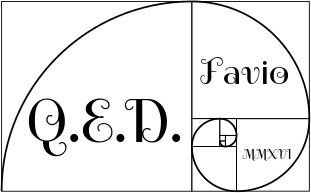
\includegraphics[scale=0.2]{logoQED}

\textbf{(d)} Por último hay que mostar que para distancias grandes, 
i.e. $\rho^2 + z^2 \gg a^2$, el potencial puede ser expandido en series 
de potencia para $(\rho^2 + z^2)^{-1}$, y que los términos más importantes 
de esta expansión son 

\begin{equation}
 \Phi = \frac{Va^2}{2}\frac{z}{(\rho^2 + z^2)^{3/2}}\left[1 - 
 \frac{3a^2}{4(\rho^2 + z^2)} + \frac{5(3\rho^2a^2+a^4)}{8\rho^2 + z^2)^2} 
 + \dots \right],
\end{equation}

y validar la consistencia de este resultado con lo obtenido en el anterior 
inciso en su rango común de validez. Recordemos la expresión que 
encontramos en el inciso (b) para el potencial, 

\begin{equation}
 \Phi(\mathbf{x}) = \frac{zV}{2\pi}\int_0^a\int_0^{2\pi} 
 \frac{\rho' d\phi' d\rho'}{(\rho^2 + \rho'^2 - 2\rho\rho'\cos{(\phi - \phi')} + 
 z^2)^{3/2}},
\end{equation}

primero viendo que el problema tiene simetría azimutal, podemos hacer 
el cambio de variables $\phi' \rightarrow \phi' + \phi$, y obtener 

\begin{equation}
 \Phi(\mathbf{x}) = \frac{zV}{2\pi}\int_0^a\int_0^{2\pi} 
 \frac{\rho' d\phi' d\rho'}{(\rho^2 + \rho'^2 - 2\rho\rho'\cos{\phi'} + 
 z^2)^{3/2}},
\end{equation}

ahora factorizando $(\rho^2 + z^2)^{3/2}$ nos queda 

\begin{equation}
 \Phi = \frac{zV}{2\pi}\frac{1}{(\rho^2 + z^2)^{3/2}} 
 \int_0^{2\pi}\int_0^a  \rho'd\rho'd\phi' 
 \left(1 + \frac{\rho'^2 - 2\rho\rho'\cos{\theta'}}{\rho^+z^2}\right)^{-3/2}.
\end{equation}

De acuerdo a la expansión en la serie binomial tenemos que 

\begin{equation}
 (1 + x)^n = 1 + nx + \frac{n(n-1)}{2}x^2 + \dots,
\end{equation}

por lo tanto nos queda al expandir el término en la integral del 
potencial resulta (quedándonos hasta segundo orden)

\begin{align*}
 \Phi &= \frac{zV}{2\pi}\frac{1}{(\rho^2 + z^2)^{3/2}} \int_0^{2\pi} 
 \int_0^a \rho'd\rho'd\phi' \left[1 - \frac{3}{2}(\rho^2 + z^2)^{-1} 
 (\rho'^2 - 2\rho\rho'\cos{\phi'})\right\zerodel \\
 &\left\zerodel + \frac{15}{8}(\rho^2 + z^2)^{-2} + \dots \right].
\end{align*}

Ahora podemos integrar término a término 

\begin{align*}
 \Phi &= \frac{zV}{2\pi}\frac{1}{(\rho^2 + z^2)^{3/2}}\int_0^{2\pi}
 \int_0^a \rho'd\rho'd\phi' \\
 &- \frac{3}{2}(\rho^2 + z^2)^{-1} 
 \int_0^{2\pi} \int_0^a \rho'd\rho'd\phi' [\rho'^2 - 2\rho\rho'\cos{\phi}'] \\
 &+ \frac{15}{8}(\rho^2 + z^2)^{-2} 
 \int_0^{2\pi}\int_0^a \rho'd\rho'd\phi' [\rho'^2 - 2\rho\rho'\cos{\phi}']
 + \dots,
\end{align*}

que resulta luego de integrar y evaluar los límites de integración 
en 

\begin{align*}
  \Phi = \frac{zV}{2\pi} \frac{1}{(\rho^2 + z^2)^{3/2}}\left\{[\pi a^2] - 
 \frac{3}{2}(\rho^2 + z^2)^{-1}\left[\frac{\pi}{2}a^4 \right]\right\zerodel \\
 + \left\zerodel \frac{15}{8}(\rho^2 + z^2)^{-2}\left[2\pi\frac{a^6}{6} + 
 4\pi\rho^2\frac{a^4}{4}\right] + \dots \right\},
\end{align*}

y con un poco de manipulación algebraica llegamos a 

\begin{equation}
 \boxed{\Phi = \frac{Va^2}{2}\frac{z}{(\rho^2 + z^2)^{3/2}}\left[1 - 
 \frac{3a^2}{4(\rho^2 + z^2)} + \frac{5(3\rho^2a^2+a^4)}{8(\rho^2 + z^2)^2} 
 + \dots \right]}.
 \label{eq:expansionPoten1}
\end{equation}

\hspace{10cm}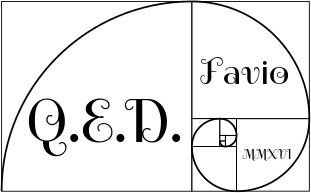
\includegraphics[scale=0.2]{logoQED}

Por último, debemos verificar que esta ecuación que acabamos de obtener 
sea equivalente a la que encontramos en el inciso anterior, es decir 
a lo largo del eje del círculo $(\rho = 0)$. Entonces haciendo $\rho = 0$ 
en \eqref{eq:expansionPoten1} obtenemos 

\begin{equation}
 \Phi = \frac{Va^2}{2}\frac{1}{z^2}
 \left[1 - \frac{3}{4}\frac{a^2}{z^2} + 
 \frac{5}{8}\frac{a^4}{z^4} + \dots \right],
\end{equation}

\begin{equation}
 \Phi = V\left[\frac{a^2}{2z^2} - 
 \frac{3}{8}\frac{a^4}{z^4} + 
 \frac{5}{16}\frac{a^6}{z^6} + \dots \right],
\end{equation}

\begin{equation}
 \therefore \Phi = V\left[1 - \left(1 - \frac{a^2}{2z^2} - 
 \frac{3}{8}\frac{a^4}{z^4} + 
 \frac{5}{16}\frac{a^6}{z^6} + \dots  \right) \right],
\end{equation}

y recordando la expansión $(1 + x)^{-1/2} = 1 - \frac{1}{2}x + 
\frac{3}{8}x^2 - \frac{5}{16}x^3 + \dots$, donde $x \rightarrow a^2/z^2$, 
nos queda 

\begin{equation*}
 \Phi = V\left[1 - \left(1 + \frac{a^2}{z^2} \right)^{-1/2} \right] = 
 V\left[1 - \left(\frac{a^2+z^2}{z^2} \right)^{-1/2} \right] = 
 V\left[1 - \left(\frac{(a^2+z^2)^{-1/2}}{z^{-1}} \right) \right],
\end{equation*}

\begin{equation}
 \boxed{\therefore \Phi = V \left[1 - \frac{z}{\sqrt{a^2 + z^2}} \right]}.
\end{equation}

\hspace{10cm}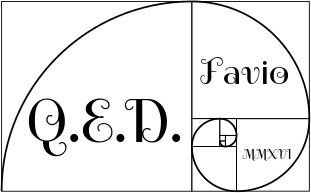
\includegraphics[scale=0.2]{logoQED}

\section{Problema 4. Problema 2.5 de Classical Electrodynamics (2da edición) de Jackson 
\cite{jackson2} y 2.9 (3ra edición) de Jackson \cite{jackson3}.}

Una concha conductora, aislada y esférica de radio $a$ está en un campo eléctrico 
uniforme $E_0$. Si la esfera es cortada en dos hemisferios por un plano perpendicular 
al campo, encuentre la fuerza requerida para prevenir que los hemisferios se 
separen 

\begin{enumerate}[label=\textbf{(\alph*)}]
 \item si la concha no tiene carga;
 \item si la carga total en la concha es $Q$.
\end{enumerate}

\vspace{.3cm}

\underline{Solución:} \vspace{.3cm}

\section{Problema 5. Problema 2.6 de Classical Electrodynamics (2da edición) de Jackson 
\cite{jackson2} y 2.10 (3ra edición) de Jackson \cite{jackson3}.}

Un capacitor de placas paralelas grande está hecho de dos láminas conductoras 
planas con una separación $D$, una de ellas tiene tiene un bulto semiesférico 
de radio $a$ en su superficie interna $(D \gg a)$. El conductor con el bulto 
es puesto a un potencial cero, y el otro conductor es a un potencial tal que, 
lejos del bulto, el campo eléctrico entre las placas es $E_0$.

\begin{enumerate}[label=\textbf{(\alph*)}]
 \item Calcule la densidad de carga superficial en un punto arbitrario del 
 plano y sobre el bulto, y esboce su comportamiento como una función de la distancia 
 (o ángulo).
 \item Muestre que la carga total en el bulto tiene la magnitud $3\pi\epsilon_0E_0a^2$.
 \item Si, en cambio de tener la otra lámina a un potencial diferente, una carga 
 puntual $q$ es colocada directamente arriba del bulto semiesférico a una distancia 
 $d$ de su centro, muestre que la carga inducida sobre el bulto es 
 $$
 q' = -q\left[1 - \frac{d^2 - a^2}{d\sqrt{d^2 + a^2}} \right]
 $$
\end{enumerate}

\vspace{.3cm}

\underline{Solución:} \vspace{.3cm}

\begin{thebibliography}{10}
\bibitem{jackson2}
J. Jackson, \emph{Classical Electrodynamics}, 2da edición. John Wiley and Sons, Inc. 
1975.
\bibitem{jackson3}
J. Jackson, \emph{Classical Electrodynamics}, 3ra edición. John Wiley and Sons, Inc. 
1999.
\bibitem{griffiths}
D. Griffits, \emph{Introduction to Electrodynamics}, 4ta edición, Pearson Education, 
2013.
\end{thebibliography}

\end{document}